\section{Dormand-Prince 5(4)}
We consider again the initial value problem in (\ref{2_problem}).

\subsection{Describe the Dormand-Prince (DOPRI54) method with adaptive time step size}
The DOPRI54 method is an explicit method of the Runge-Kutta family of ODE solvers. The method calculates a fourth- and fifth-order accurate solutions. The difference between them is used as an approximation of the local truncation error. Note that this approximation is obtained by only using an extra function evaluation, avoiding all the computational costs of other ways of approximating it (f.e. the step doubling we used in all the adaptive implementations before). This behaviour makes the DOPRI54 a very solid choice as an adaptive ODE solver. 

\begin{table}[H]
\centering
\begin{tabular}{c|ccccccc}
0    &            &             &            &          &               &          &      \\
1/5  & 1/5        &             &            &          &               &          &      \\
3/10 & 3/40       & 9/40        &            &          &               &          &      \\
4/5  & 44/45      & -56/15      & 32/9       &          &               &          &      \\
8/9  & 19372/6561 & -25360/2187 & 64448/6561 & -212/729 &               &          &      \\
1    & 9017/3168  & -355/33     & 46732/5247 & 49/176   & -5103/18656   &          &      \\
1    & 35/384     & 0           & 500/1113   & 125/192  & -2187/6784    & 11/84    &      \\ \hline
     & 35/384     & 0           & 500/1113   & 125/192  & -2187/6784    & 11/84    & 0    \\
     & 5179/57600 & 0           & 7571/16695 & 393/640  & -92097/339200 & 187/2100 & 1/40
\end{tabular}
\caption{Butcher Tableau of the Dormand-Prince 5(4) method}
\label{DOPRI54_Tableau}
\end{table}

%%%%%%%%%%%%%%%%%%%%%%%%%%%%%%%%%%%%%%%%%%%%%%%%%%%%%%%%%%%%%%%%%%%%%%%%%%%%%%%%%%%%%%%%%%%%%%%%%%%
\subsection{Implement an algorithm in Matlab for the DOPRI54 method with adaptive time step size. Provide the code in your report.  Use a format that enables syntax highlighting. Comment on the code}
\begin{lstlisting}[caption = Dormand-Prince 5(4) method with adaptive time step size, captionpos=b, label=7_DOPRI54_adaptive]
function [T_out,X_out,e_out,r_out,h_out,info] = DOPRI54_adaptive(fun,tspan,h0,x0,abstol,reltol,butcher,args)

% Controller parameters
epstol = 0.8;
kpow = 1/6;
facmin = 0.1;
facmax = 5.0;

t0 = tspan(1);
tf = tspan(end);
t = t0;
h = h0;
x = x0;

nx = size(x0,1);

T_out = t0;
X_out = x0;
e_out = zeros(nx,1);
r_out = [];
h_out = [];
info = zeros(4,1);

nfun = 0;
nstep = 0;
naccept = 0;

% Extract Butcher Tableau
s = butcher.stages;
AT = butcher.AT;
b = butcher.b;
c = butcher.c;
d = butcher.d;

% Allocate memory for the stages
T = zeros(1,s);
X = zeros(nx,s);
F = zeros(nx,s);

while t < tf
    
    % Size of last step
    if t+h > tf
        h = tf - t;
    end
    % First stage
    T(1) = t;
    X(:,1) = x;
    F(:,1) = feval(fun,T(1),X(:,1),args{:});
    nfun = nfun + 1;
    
    AcceptStep = false;
   
    while ~AcceptStep
        % Precalculated parameters
        hAT = h*AT;
        hb = h*b;
        hc = h*c;
        hd = h*d;

        % Following stages
        for i = 2:s
            T(i) = t + hc(i);
            X(:,i) = x + F(:,1:i-1)*hAT(1:i-1,i);
            F(:,i) = feval(fun,T(i),X(:,i),args{:});
            nfun = nfun + 1;
        end
        
        % Error estimation
        e = F*hd;
        xhat = x + F*hb;
        r = max(abs(e)./max(abstol,abs(xhat).*reltol));
         % Check conditon
        AcceptStep = r <=1;
        
        if AcceptStep
            t = t+h;
            x = xhat;
            
            T_out = [T_out,t];
            X_out = [X_out,x];
            e_out = [e_out,e];
            r_out = [r_out, r];
            h_out = [h_out, h];
            naccept = naccept + 1;
        end
        
        % step size controller (Asymptotic or second order PI)
        h = max(facmin,min((epstol/r)^kpow,facmax))*h;
        nstep = nstep+1;    
    end
end

info(1) = nfun;
info(2) = nstep;
info(3) = naccept;
info(4) = nstep - naccept;

end
\end{lstlisting}

%%%%%%%%%%%%%%%%%%%%%%%%%%%%%%%%%%%%%%%%%%%%%%%%%%%%%%%%%%%%%%%%%%%%%%%%%%%%%%%%%%%%%%%%%%%%%%%%%%%
\subsection{Test your problem for test equation. Discuss order and stability of the numerical method}
We will proceed testing the Dormand-Prince 5(4) method in a similar manner as we did for the classical Runge-Kutta method (RK4) in part \ref{part5}. The method has order 5 but, as the asked implementation is only for an adaptive method we can't show the same plots as for the fixe Runge-Kutta.
The shape of the local and global errors vs. time is similar to the one obtained for the adaptive classical Runge-Kutta in Figure \ref{6_3_TE}. Weirdly, the solution for the Dormand-Prince 5(4) has slightly more error. It's also worth noticing that the approximation of the error of the method is larger than the real local error, which is a nice thing. 

\begin{figure}[H]
    \centering
    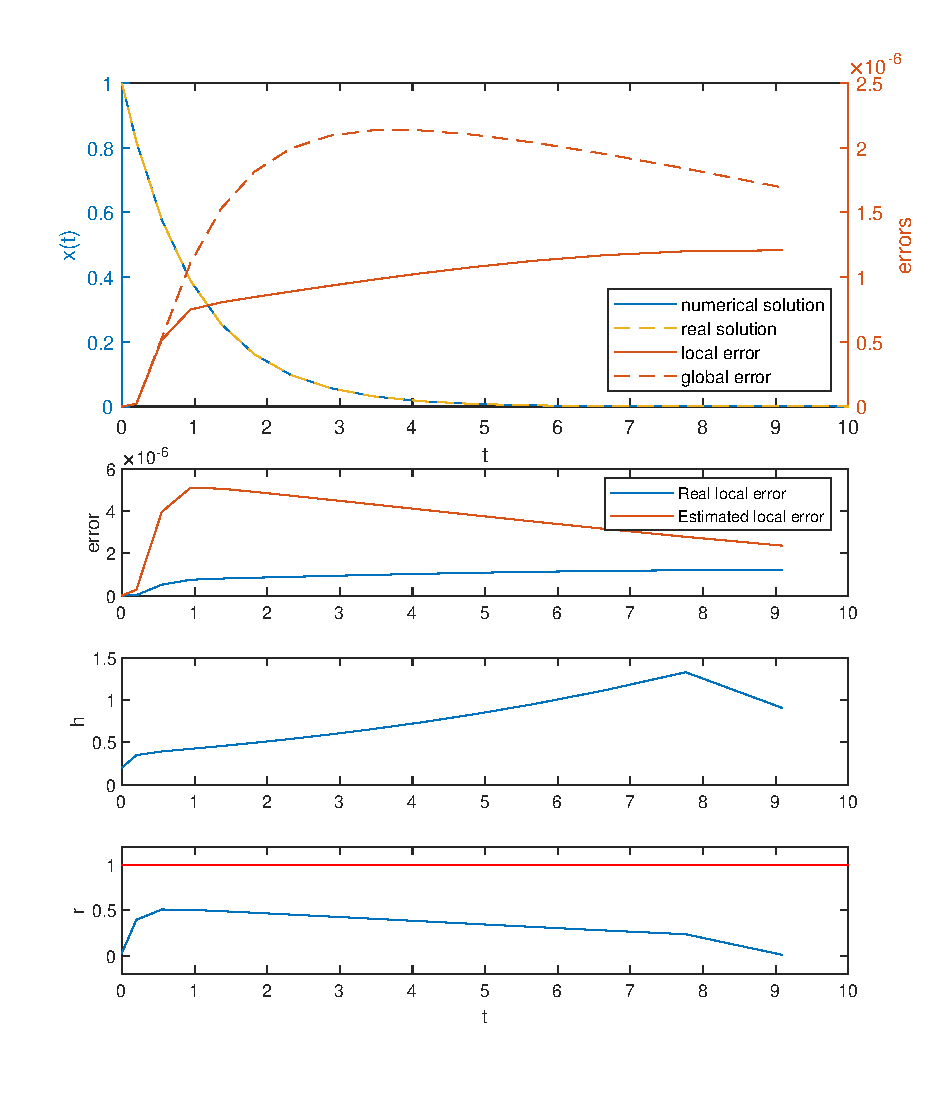
\includegraphics[width=0.7\linewidth]{images/7/7_3_TestEquation.pdf} 
    \caption{Solution and errors vs. time for the Test equation using adaptive Dormand-Prince 5(4) method}
    \label{7_3_TE}
\end{figure}

\begin{figure}[H]
\centering
    \begin{subfigure}{0.49\linewidth}
        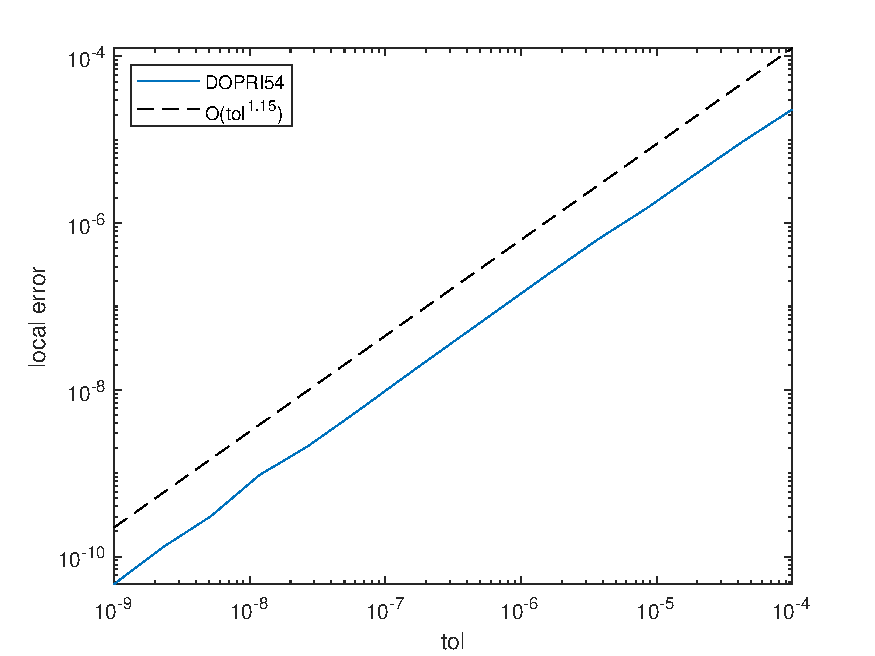
\includegraphics[width=\linewidth]{images/7/7_3_localerror.pdf}
        \caption{Local error}
    \end{subfigure}
    \begin{subfigure}{0.49\linewidth}
        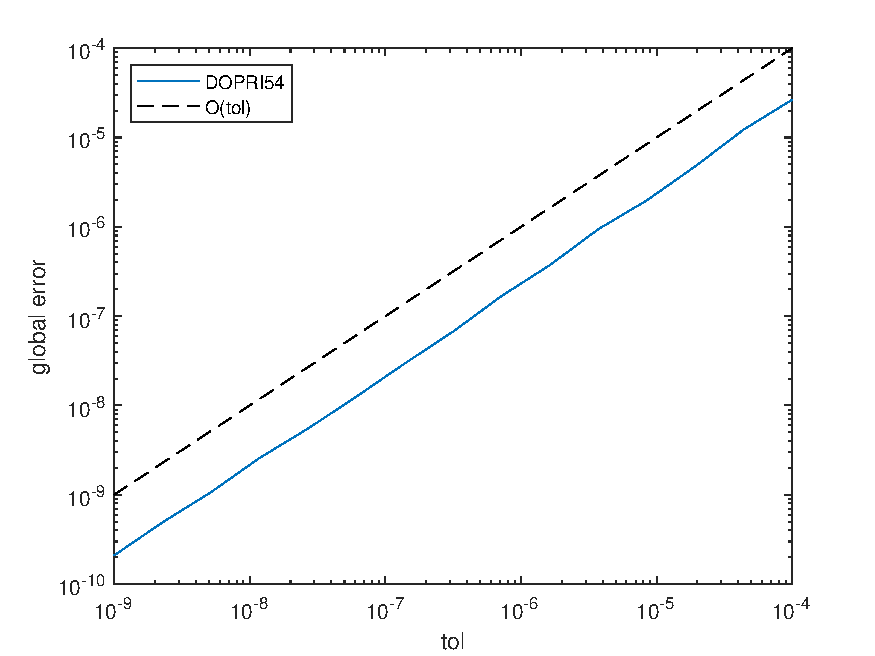
\includegraphics[width=\linewidth]{images/7/7_3_globalerror.pdf}
        \caption{Global error}
    \end{subfigure}
    \caption{Local and global errors vs. tolerances for the Test equation using adaptive Dormand-Prince 5(4) method}
    \label{7_3_TE_errors}
\end{figure}

For the stability of the method, the solution of a member of the Runge-Kutta family of ODE solvers for the test equation is given as:
\begin{equation*}
    x_{n+1} = R(h \lambda) x_n \hspace{1em} R(z) = 1 + z b'(I-zA)^(-1)e,
\end{equation*}
where, A and b are the top right matrix and the bottom right vector in the Butcher Tableau \ref{DOPRI54_Tableau}. The stability regions for complex values of $h\lambda$ are shown in Figure \ref{7_3_stability_regions}. Here we can observe that the method is neither A-stable, nor L-stable, given that there are regions on the left side plane that are greater than 1 and that $\lim_{z \to -\infty}|R(z)| \neq 0$.

\begin{figure}[H]
    \centering
    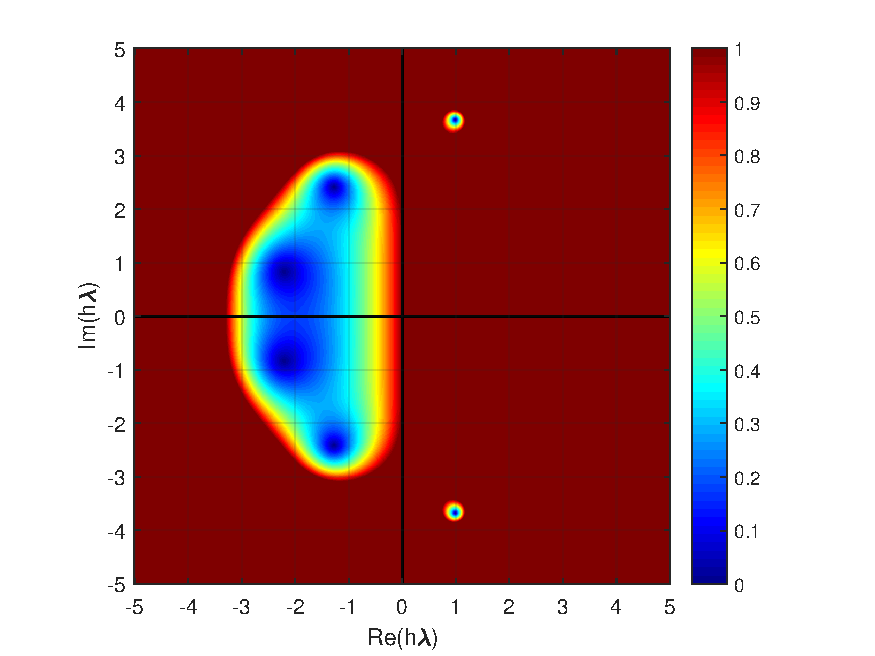
\includegraphics[width=0.7\linewidth]{images/7/7_3_stability_regions.pdf} 
    \caption{Values of $R(h\lambda)$ for the Dormand-Prince 5(4) method}
    \label{7_3_stability_regions}
\end{figure}

\pagebreak

%%%%%%%%%%%%%%%%%%%%%%%%%%%%%%%%%%%%%%%%%%%%%%%%%%%%%%%%%%%%%%%%%%%%%%%%%%%%%%%%%%%%%%%%%%%%%%%%%%%
\subsection{Test your algorithms on the Van der Pol problem \texorpdfstring{($\mathbf{\mu = 1.5}$ and $\mathbf{\mu = 15}$, $\mathbf{x_0 = [1.0;1.0]}$).}{(mu = 1.5 and mu = 15, x0 = [1.0;1.0]).}}
The results for the Van der pol problem are shown below. When comparing to the Explicit Euler with adaptive results shown in Figures \ref{2_4_adaptive_mu_1_5} and \ref{2_4_adaptive_mu_15}, we can see that the method achieves better performance when working with same tolerances, or even larger. Contrary to what happened for the classical Runge-Kutta, the shift of frequency of the signals has reappeared completely and bigger tolerances don't work as good as before. Here we can observe a pretty strange behaviour, the biggest tolerance solution shifts negatively at some points. Also, as it's an explicit method, it's still sensible to the stiffness of the Van der Pol with $\mu=15$, although it handles the change in step size a lot better than the other ones. 

Finally, comparing both tables with the results from the adaptive classical Runge-Kutta (Tables \ref{6_4_adaptive_mu_1_5_table} and \ref{6_4_adaptive_mu_15_table}) we observe that, although the number of calculated steps is similar, the number of function evaluations is considerably lower in the Dormand-Prince 5(4), due to the way of calculating an approximate local error and not using step doubling.

\begin{figure}[H]
    \centering
    \makebox[\textwidth][c]{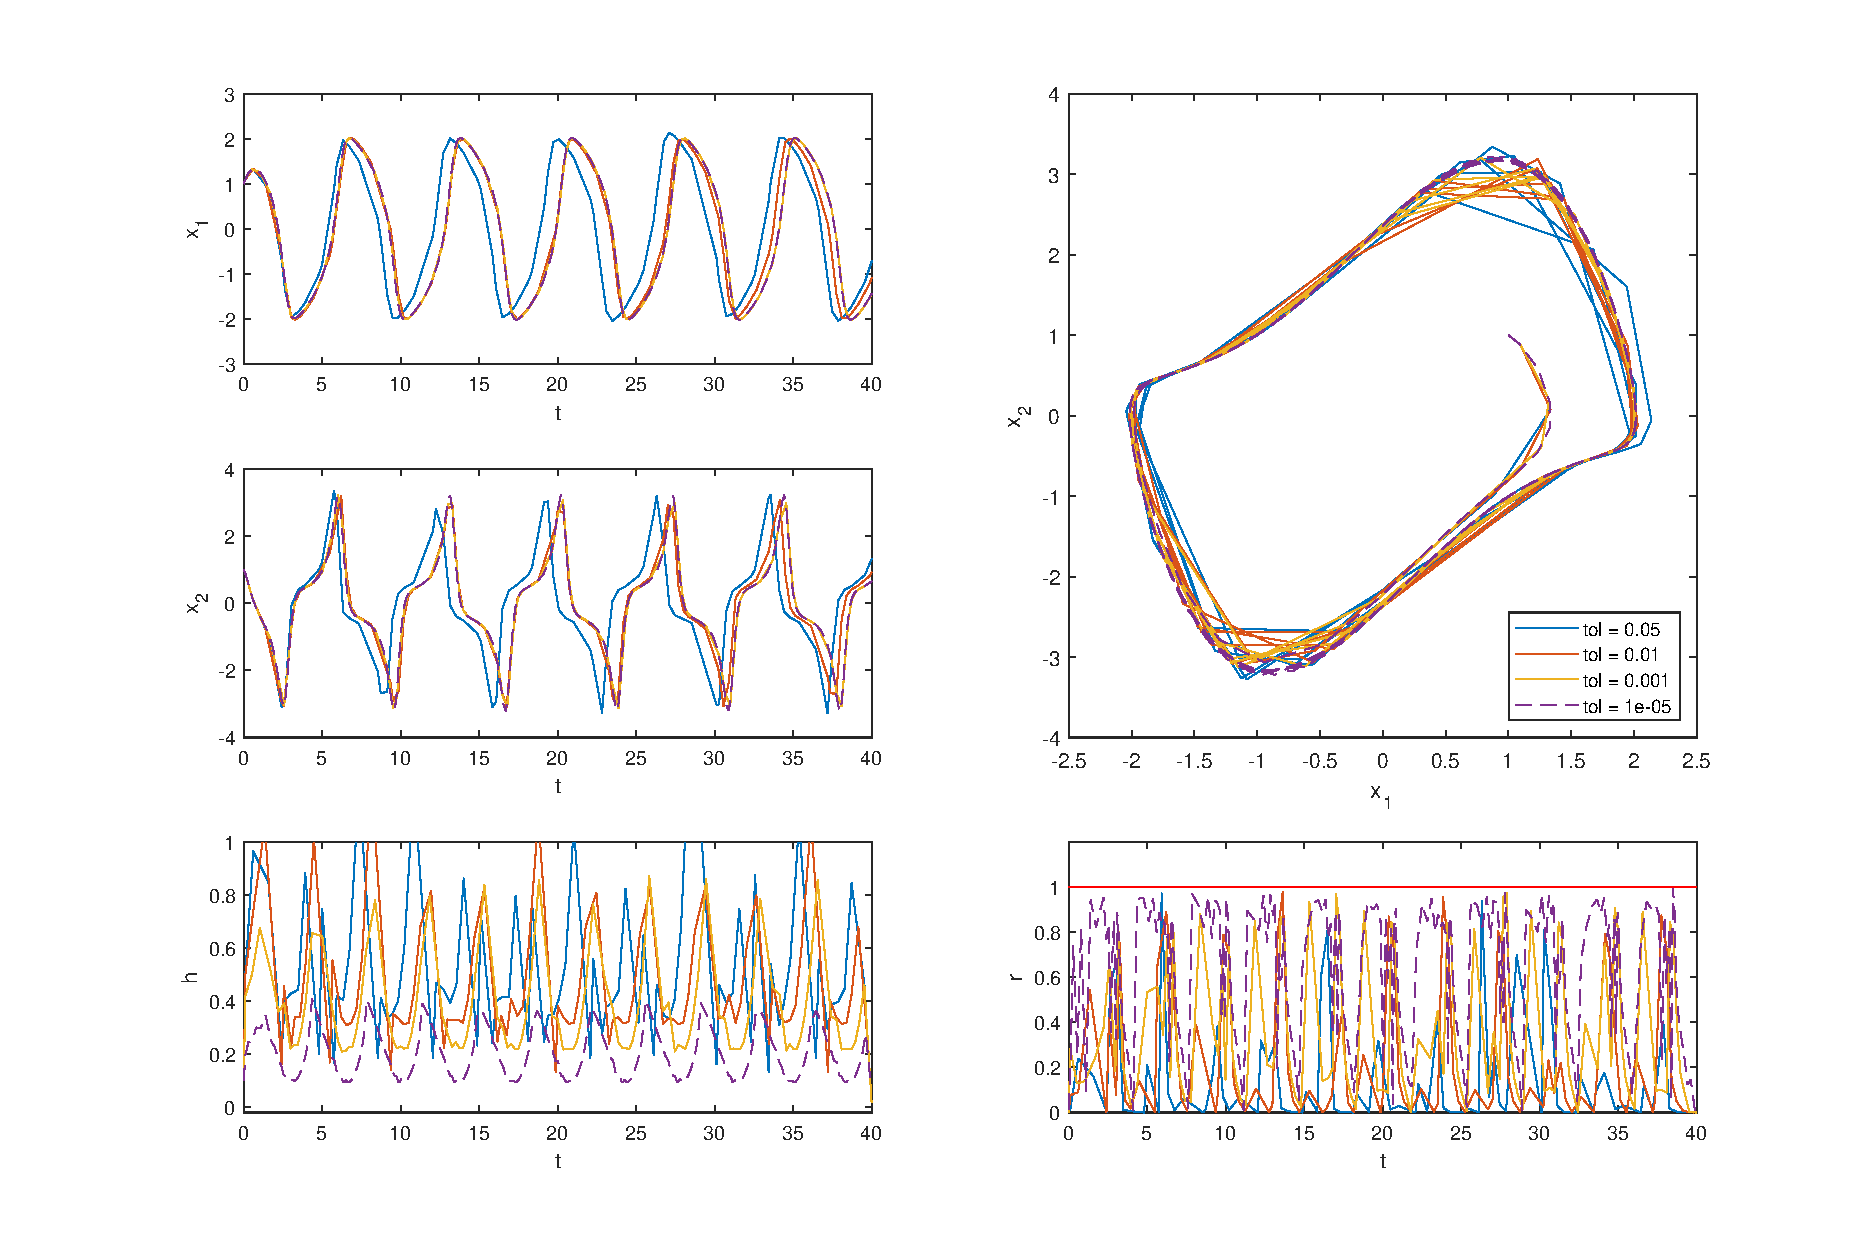
\includegraphics[width=1.25\textwidth]{images/7/7_4_adaptive_mu_1_5.pdf}}
    \caption{Solution for the Van der Pol problem ($\mathit{\mu = 1.5}$) using Dormand-Prince 5(4) with adaptive step size}
    \label{7_4_mu_1_5}
\end{figure}

\begin{table}[H]
    \centering
    \begin{tabular}{@{}l|cccc@{}}
    \toprule
    Tolerances           & 0.05 & 0.01 & 0.001 & 1e-05 \\ \midrule
    Function evaluations & 867  & 936  & 1194  & 2350  \\
    Calculated steps     & 131  & 141  & 180   & 352   \\
    Accepted steps       & 81   & 90   & 114   & 238   \\
    Rejected steps       & 50   & 51   & 66    & 114   \\ \bottomrule
    \end{tabular}
    \caption{Parameters of the Dormand-Prince 5(4) with adaptive step size for the Van der Pol problem ($\mathit{\mu = 1.5}$)}
    \label{7_4_adaptive_mu_1_5_table}
\end{table}

\begin{figure}[H]
    \centering
    \makebox[\textwidth][c]{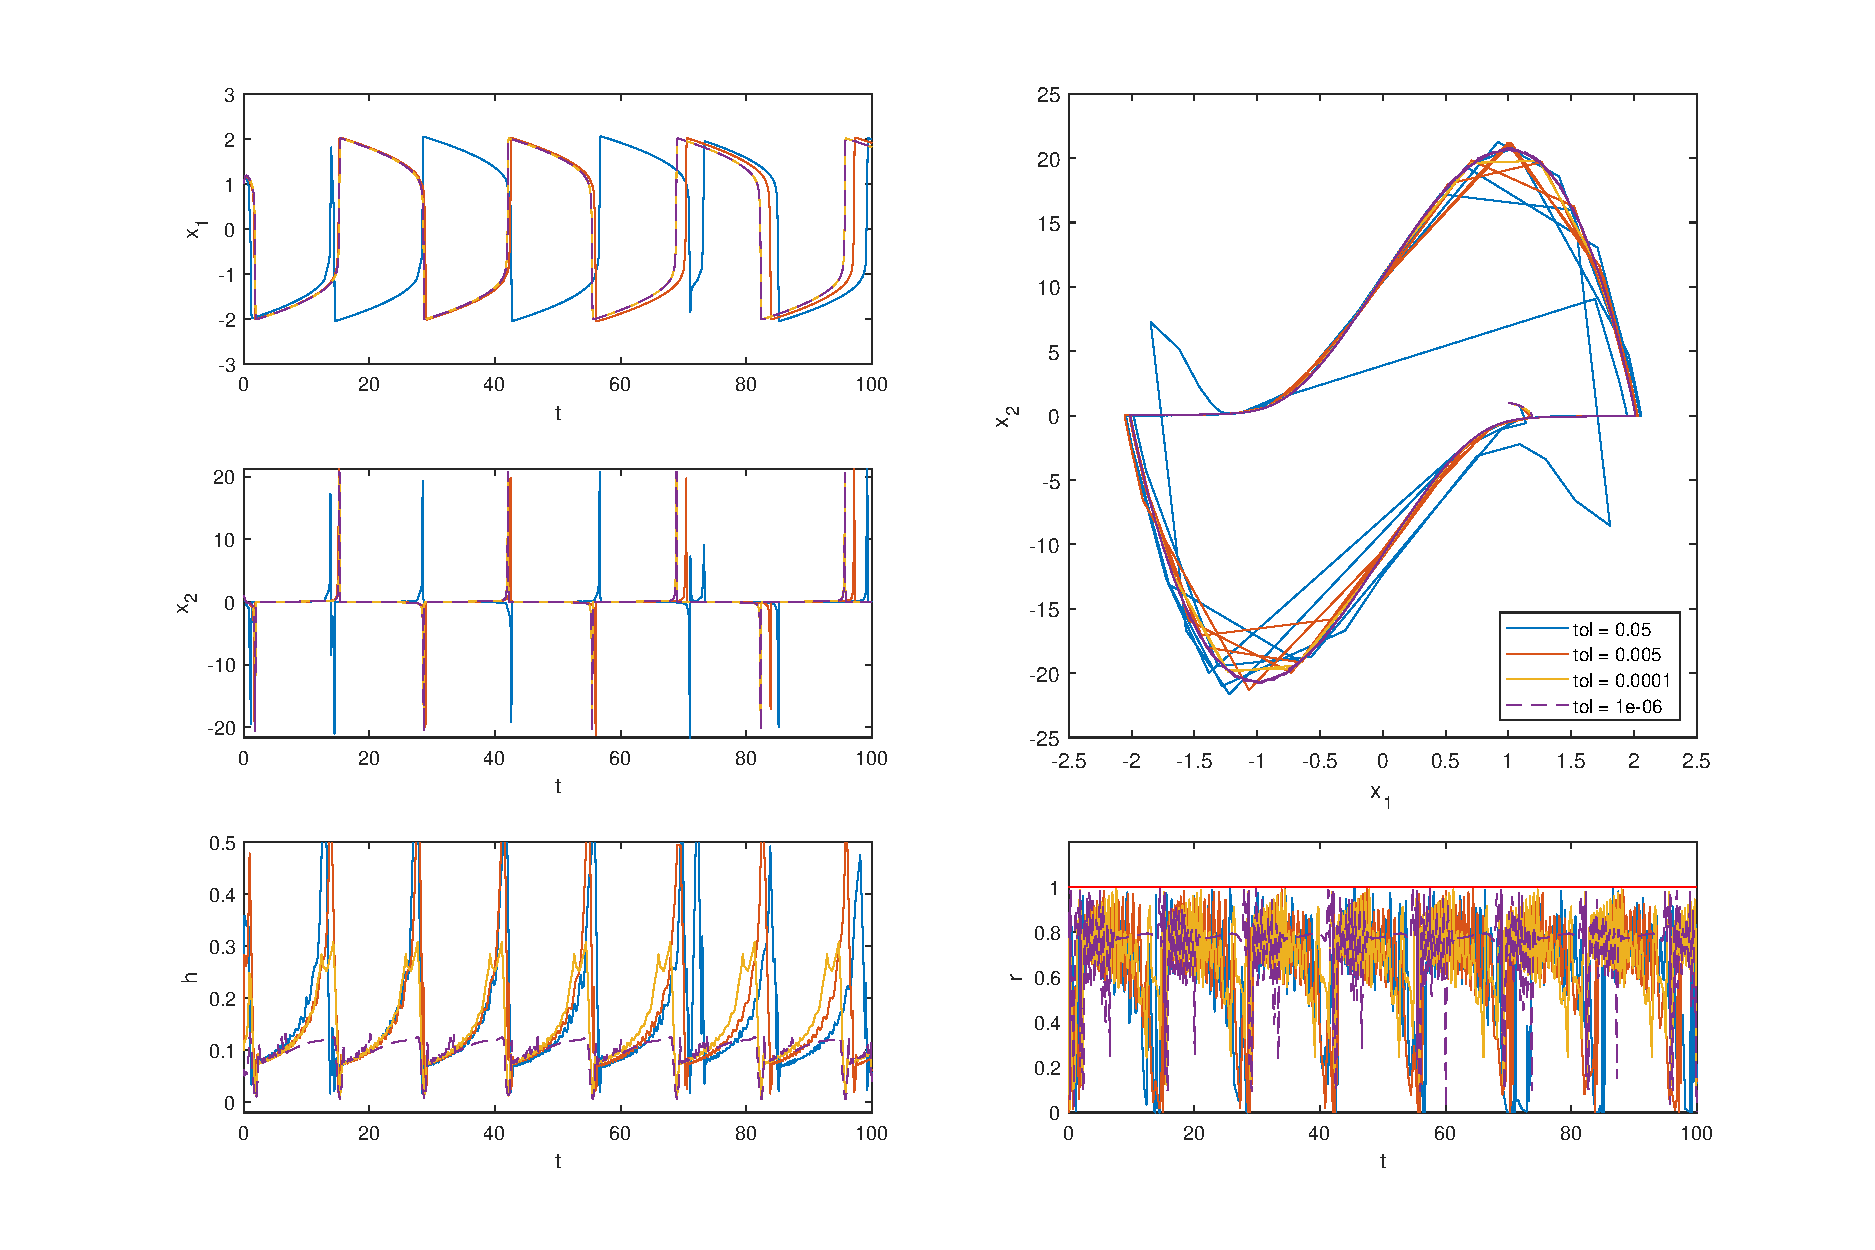
\includegraphics[width=1.25\textwidth]{images/7/7_4_adaptive_mu_15.pdf}}
    \caption{Solution for the Van der Pol problem ($\mathit{\mu = 15}$) using Dormand-Prince 5(4) with adaptive step size}
    \label{7_4_mu_15}
\end{figure}

\begin{table}[H]
    \centering
    \begin{tabular}{@{}l|cccc@{}}
    \toprule
    Tolerances           & 0.05 & 0.005 & 0.0001 & 1e-06 \\ \midrule
    Function evaluations & 6729 & 6624  & 7590   & 10998 \\
    Calculated steps     & 979  & 959   & 1106   & 1608  \\
    Accepted steps       & 855  & 870   & 954    & 1350  \\
    Rejected steps       & 124  & 89    & 152    & 258   \\ \bottomrule
    \end{tabular}
    \caption{Parameters of the Dormand-Prince 5(4) with adaptive step size for the Van der Pol problem ($\mathit{\mu = 15}$)}
    \label{7_4_adaptive_mu_15_table}
\end{table}

%%%%%%%%%%%%%%%%%%%%%%%%%%%%%%%%%%%%%%%%%%%%%%%%%%%%%%%%%%%%%%%%%%%%%%%%%%%%%%%%%%%%%%%%%%%%%%%%%%%
\subsection{Test  your  algorithms  on  the  adiabatic  CSTR  problem  described  in  the papers uploaded to Learn (3D-version and 1D-version).}
Again, as in the Van der Pol, we need to set the tolerance a bit lower than in the classical Runge-Kutta for it to converge. However, it deals a lot better with the stiff area of the problem, specially for the 3D case. Again, we observe by comparing the tables that for the same number of calculated steps we need a lot less function evaluations.

\begin{figure}[H]
    \centering
    \makebox[\textwidth][c]{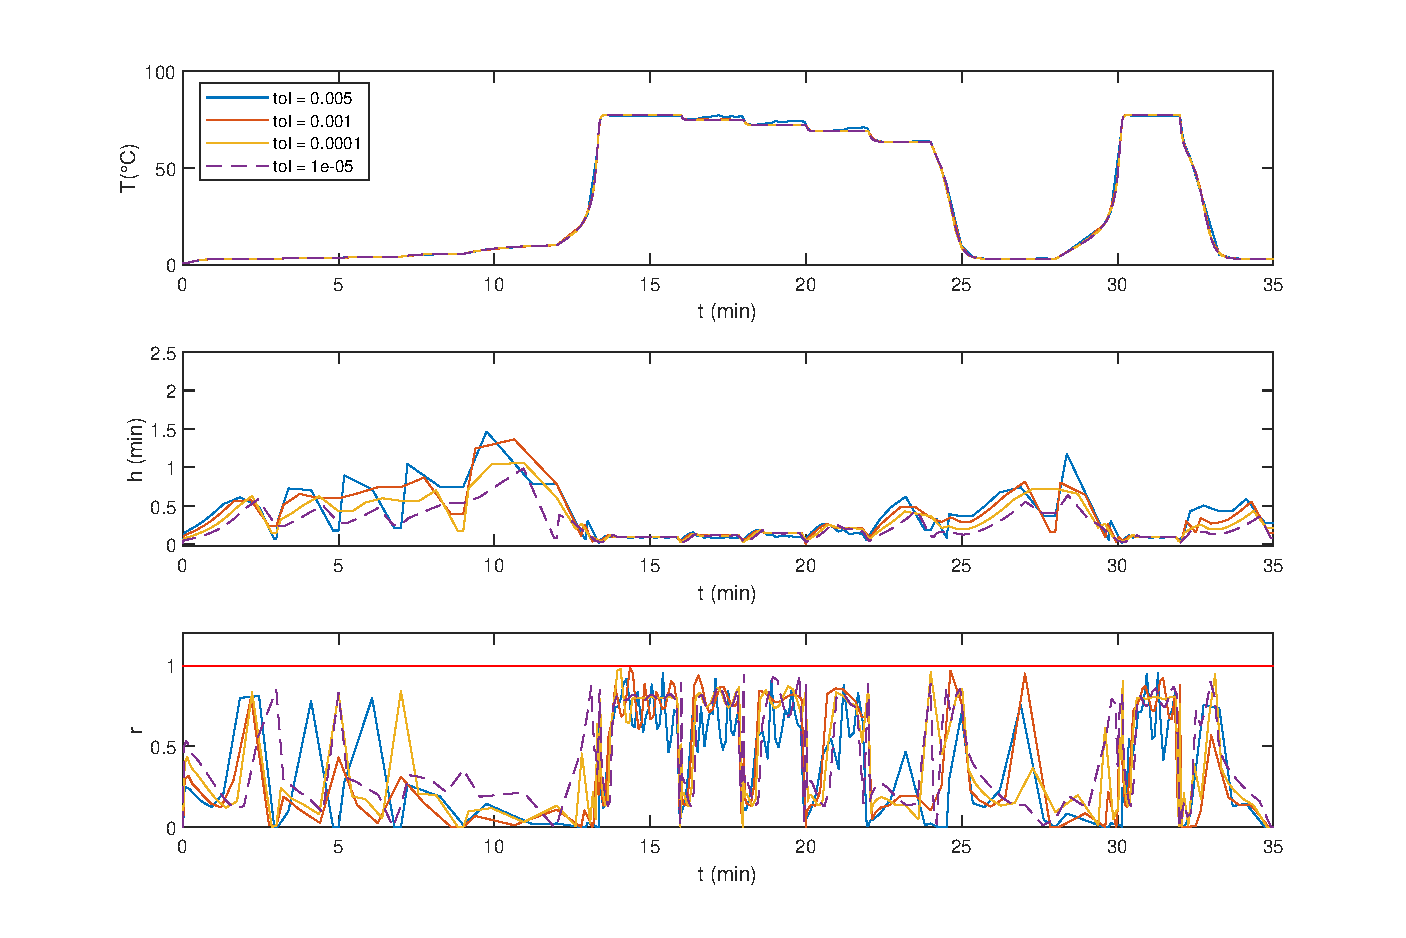
\includegraphics[width=1\textwidth]{images/7/7_5_3D_tols.pdf}}
    \caption{Solution for the CSTR 3D problem using Dormand-Prince 5(4) with adaptive step size}
    \label{7_5_3D_tols}
\end{figure}

\begin{table}[H]
    \centering
    \begin{tabular}{@{}l|cccc@{}}
    \toprule
    Tolerances           & 0.005 & 0.001 & 0.0001 & 1e-05 \\ \midrule
    Function evaluations & 1507  & 1423  & 1538   & 1918  \\
    Calculated steps     & 223   & 209   & 225    & 281   \\
    Accepted steps       & 169   & 169   & 188    & 232   \\
    Rejected steps       & 54    & 40    & 37     & 49    \\ \bottomrule
    \end{tabular}
    \caption{Parameters of the Dormand-Prince 5(4) with adaptive step size for the CSTR 3D problem}
    \label{7_5_3D_tols_table}
\end{table}

\begin{figure}[H]
    \centering
    \makebox[\textwidth][c]{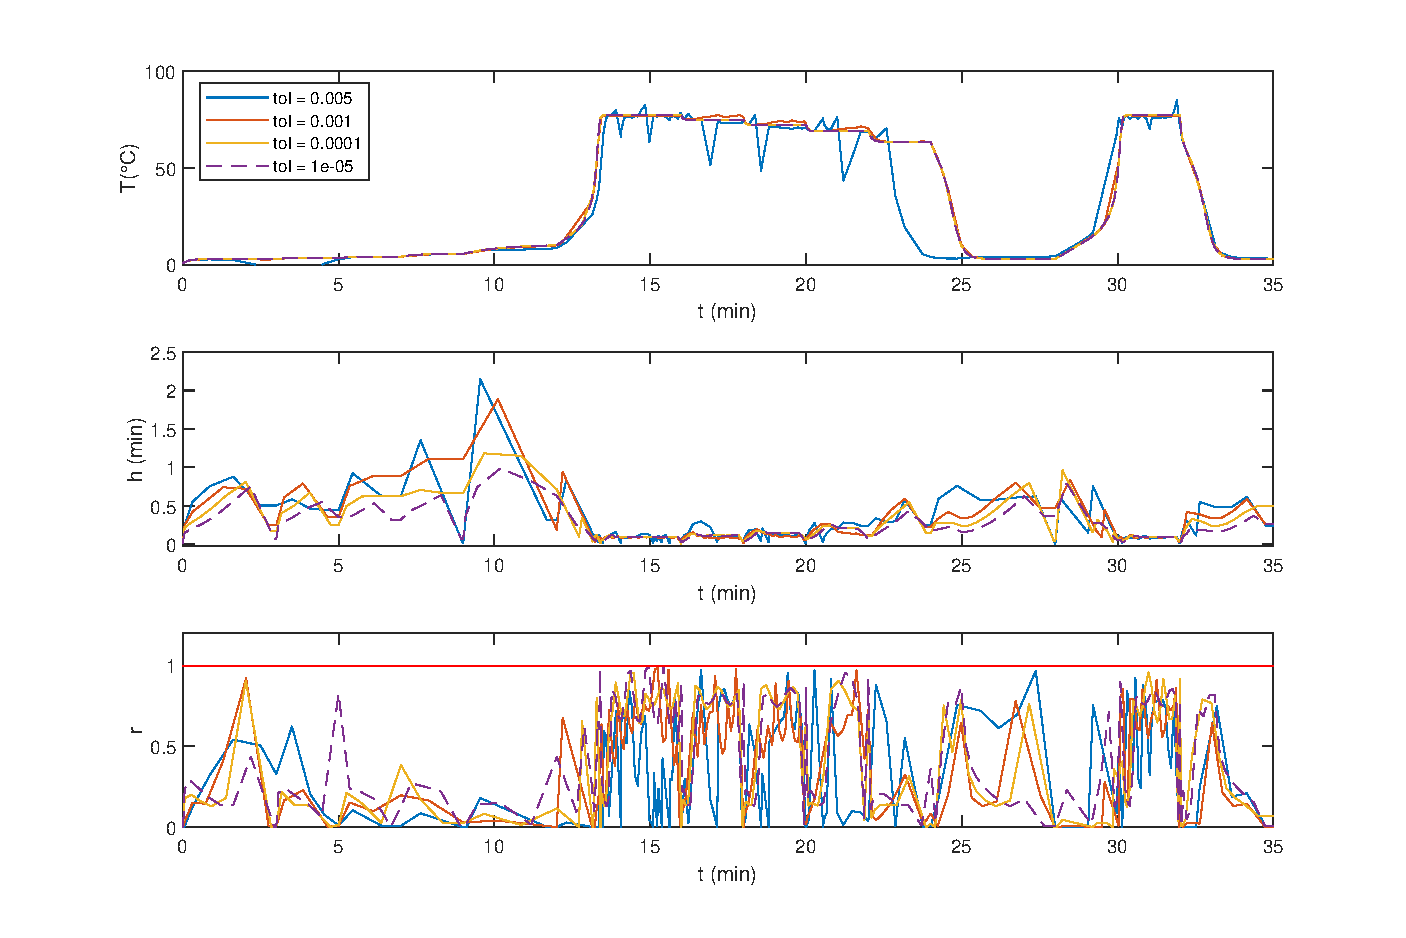
\includegraphics[width=1\textwidth]{images/7/7_5_1D_tols.pdf}}
    \caption{Solution for the CSTR 1D problem using Dormand-Prince 5(4) with adaptive step size}
    \label{7_5_1D_tols}
\end{figure}

\begin{table}[H]
    \centering
    \begin{tabular}{@{}l|cccc@{}}
    \toprule
    Tolerances           & 0.005 & 0.001 & 0.0001 & 1e-05 \\ \midrule
    Function evaluations & 1397  & 1441  & 1408   & 1637  \\
    Calculated steps     & 206   & 213   & 206    & 240   \\
    Accepted steps       & 161   & 163   & 172    & 197   \\
    Rejected steps       & 45    & 50    & 34     & 43    \\ \bottomrule
    \end{tabular}
    \caption{Parameters of the Dormand-Prince 5(4) with adaptive step size for the CSTR 1D problem}
    \label{7_5_1D_tols_table}
\end{table}

%%%%%%%%%%%%%%%%%%%%%%%%%%%%%%%%%%%%%%%%%%%%%%%%%%%%%%%%%%%%%%%%%%%%%%%%%%%%%%%%%%%%%%%%%%%%%%%%%%%
\subsection{Compare the results from your algorithms with the results you get using some of Matlab's ODE solvers (in particular ode45 which implements the DOPRI54 method)}

For the Van der Pol problem, we tested the Dormad-Prince 4(5) method against \code{ode45} for the non-stiff case ($\mu = 1.5$), and against \code{ode15s} for the stiff case ($\mu = 15$). With this method, should be expecting a similar performance, if not exact same to the \code{ode45}, as the Matlab documentation says this is their implemented method. However, the results we obtain are actually different. This could be caused because Matlab implementation uses a different way of calculating the error other than the approximation from the method, or that we forgot to adjust some of the flags other than the actual tolerances. 

In the results, the Dormand-Prince achieves same accuracy as the \code{ode45}. IN the number of function evaluations though, we see a difference. For the Van der Pol it has a little bit more, but in the CSTR it has a lot less function evaluations. Their performance for this problem is also quite similar. As it's an explicit method, \code{ode15s} still remains the best choice for the stiff case, when looking at the number of function evaluations.

\begin{figure}[H]
    \centering
    \makebox[\textwidth][c]{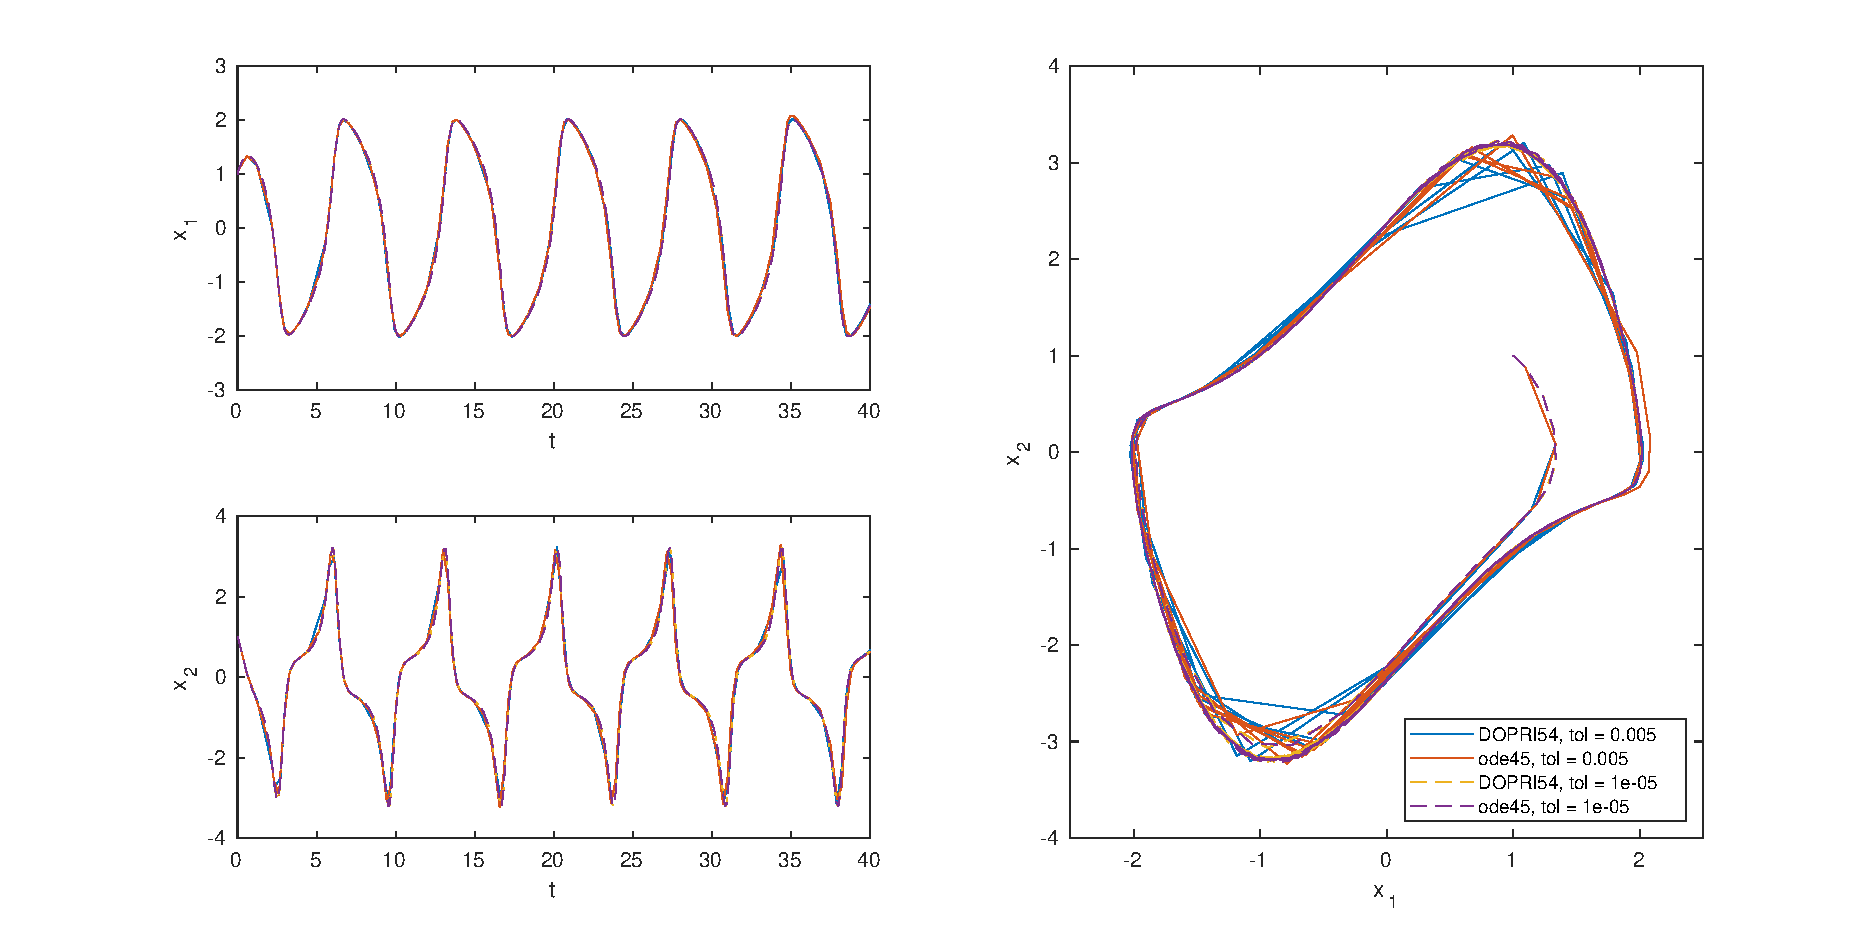
\includegraphics[width=1.25\textwidth]{images/7/7_6_mu_1_5.pdf}}
    \caption{Solution for the Van der Pol problem ($\mathit{\mu = 1.5}$) using Dormand-Prince 5(4) vs. \code{ode45}}
    \label{7_6_mu_1_5}
\end{figure}

\begin{table}[H]
    \centering
    \begin{tabular}{@{}l|cc|cc@{}}
    \toprule
    \textbf{Method}      & \multicolumn{2}{c|}{\textbf{DOPRI45}} & \multicolumn{2}{c}{\textbf{ode45}} \\
    Tolerances           & 0.005             & 1e-05             & 0.005            & 1e-05           \\ \midrule
    Function evaluations & 960               & 2350              & 793              & 1903            \\
    Calculated steps     & 144               & 352               & 132              & 317             \\
    Accepted steps       & 96                & 238               & 103              & 270             \\
    Rejected steps       & 48                & 114               & 29               & 47              \\ \bottomrule
    \end{tabular}
    \caption{Parameters of the Dormand-Prince 5(4) vs. \code{ode45} for the Van der Pol problem ($\mathit{\mu = 1.5}$)}
    \label{7_6_adaptive_mu_1_5_table}
\end{table}

\begin{figure}[H]
    \centering
    \makebox[\textwidth][c]{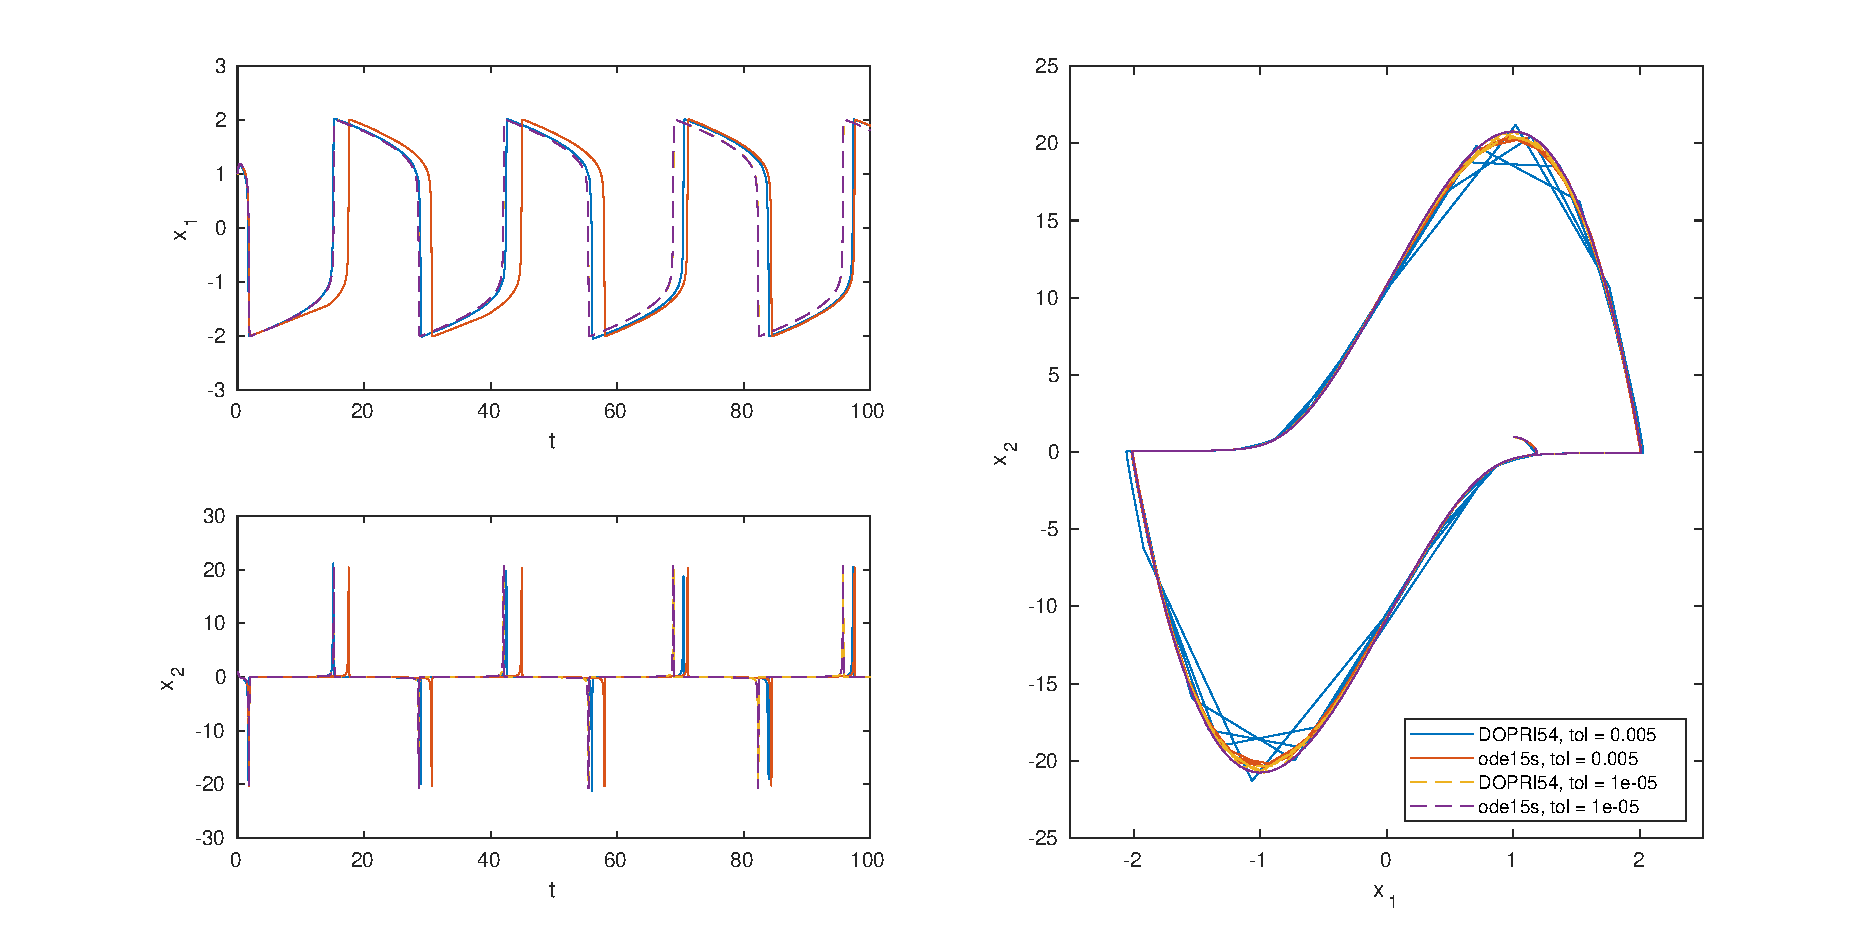
\includegraphics[width=1.25\textwidth]{images/7/7_6_mu_15.pdf}}
    \caption{Solution for the Van der Pol problem ($\mathit{\mu = 15}$) using Dormand-Prince 5(4) vs. \code{ode15s}}
    \label{7_6_mu_15}
\end{figure}

\begin{table}[H]
    \centering
    \begin{tabular}{@{}l|cc|cc@{}}
    \toprule
    \textbf{Method}      & \multicolumn{2}{c|}{\textbf{DOPRI45}} & \multicolumn{2}{c}{\textbf{ode15s}} \\
    Tolerances           & 0.005             & 1e-05             & 0.005            & 1e-05            \\ \midrule
    Function evaluations & 6612              & 8728              & 1538             & 3364             \\
    Calculated steps     & 957               & 1273              & 670              & 1699             \\
    Accepted steps       & 870               & 1090              & 499              & 1456             \\
    Rejected steps       & 87                & 183               & 171              & 243              \\ \bottomrule
    \end{tabular}
    \caption{Parameters of the Dormand-Prince 5(4) vs. \code{ode15s} for the Van der Pol problem ($\mathit{\mu = 15}$)}
    \label{7_6_adaptive_mu_15_table}
\end{table}

\begin{figure}[H]
    \centering
    \begin{subfigure}{0.8\linewidth}
        \centering
        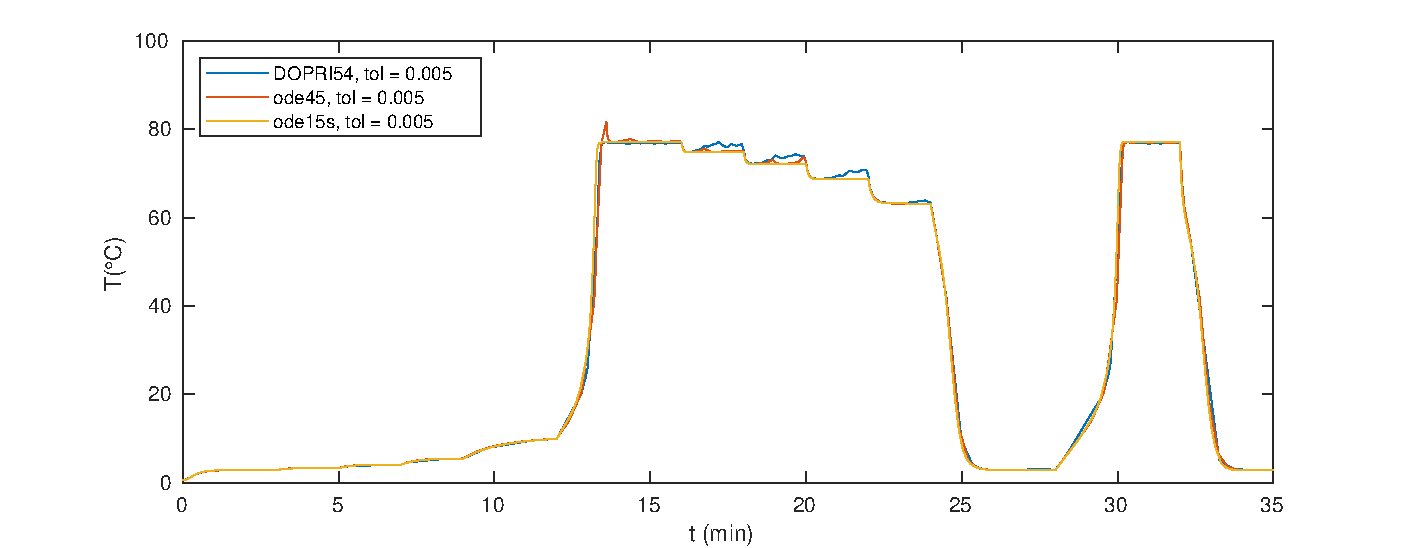
\includegraphics[width=1\linewidth]{images/7/7_6_3D.pdf} 
        \caption{CSTR 3D problem}
    \end{subfigure} \\
    \begin{subfigure}{0.8\linewidth}
        \centering
        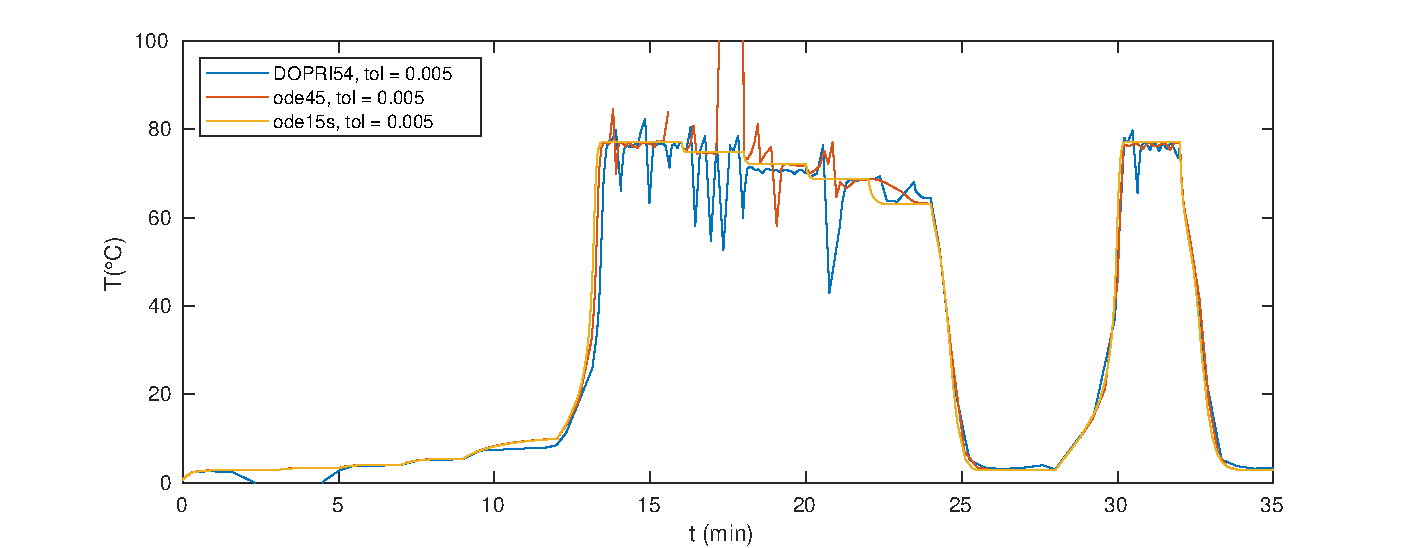
\includegraphics[width=1\linewidth]{images/7/7_6_1D.pdf}
        \caption{CSTR 1D problem}
    \end{subfigure}
    \caption{Solution for the CSTR problem using Dormand-Prince 5(4) vs. \code{ode45} and \code{ode15s}}
    \label{7_6_3D_1D}
\end{figure}

\begin{table}[H]
    \centering
    \begin{tabular}{@{}l|c|c|c@{}}
    \toprule
    \textbf{Method}      & \multicolumn{1}{c|}{\textbf{DOPRI45}} & \multicolumn{1}{c|}{\textbf{ode45}} & \multicolumn{1}{c}{\textbf{ode15s}} \\
    Tolerances           & 0.005                                 & 0.005                               & 0.005                               \\ \midrule
    Function evaluations & 1507                                  & 1285                                & 551                                 \\
    Calculated steps     & 223                                   & 1376                                & 1634                                \\
    Accepted steps       & 169                                   & 200                                 & 245                                 \\
    Rejected steps       & 54                                    & 12                                  & 31                                  \\ \bottomrule
    \end{tabular}
    \caption{Parameters of the Dormand-Prince 5(4) vs. \code{ode45} and \code{ode15s} for the CSTR-3D problem}
    \label{7_6_3D_table}
\end{table}

\begin{table}[H]
    \centering
    \begin{tabular}{@{}l|c|c|c@{}}
    \toprule
    \textbf{Method}      & \multicolumn{1}{c|}{\textbf{DOPRI45}} & \multicolumn{1}{c|}{\textbf{ode45}} & \multicolumn{1}{c}{\textbf{ode15s}} \\
    Tolerances           & 0.005                                 & 0.005                               & 0.005                               \\ \midrule
    Function evaluations & 1419                                  & 1711                                & 416                                 \\
    Calculated steps     & 210                                   & 1874                                & 1398                                \\
    Accepted steps       & 159                                   & 237                                 & 207                                 \\
    Rejected steps       & 51                                    & 46                                  & 29                                  \\ \bottomrule
    \end{tabular}
    \caption{Parameters of the Dormand-Prince 5(4) vs. \code{ode45} and \code{ode15s} for the CSTR-1D problem}
    \label{7_6_1D_table}
\end{table}
